\documentclass[11pt,]{article}
\usepackage{lmodern}
\usepackage{amssymb,amsmath}
\usepackage{ifxetex,ifluatex}
\usepackage{fixltx2e} % provides \textsubscript
\ifnum 0\ifxetex 1\fi\ifluatex 1\fi=0 % if pdftex
  \usepackage[T1]{fontenc}
  \usepackage[utf8]{inputenc}
\else % if luatex or xelatex
  \ifxetex
    \usepackage{mathspec}
  \else
    \usepackage{fontspec}
  \fi
  \defaultfontfeatures{Ligatures=TeX,Scale=MatchLowercase}
\fi
% use upquote if available, for straight quotes in verbatim environments
\IfFileExists{upquote.sty}{\usepackage{upquote}}{}
% use microtype if available
\IfFileExists{microtype.sty}{%
\usepackage{microtype}
\UseMicrotypeSet[protrusion]{basicmath} % disable protrusion for tt fonts
}{}
\usepackage[margin=1.8cm]{geometry}
\usepackage{hyperref}
\hypersetup{unicode=true,
            pdfborder={0 0 0},
            breaklinks=true}
\urlstyle{same}  % don't use monospace font for urls
\usepackage{graphicx,grffile}
\makeatletter
\def\maxwidth{\ifdim\Gin@nat@width>\linewidth\linewidth\else\Gin@nat@width\fi}
\def\maxheight{\ifdim\Gin@nat@height>\textheight\textheight\else\Gin@nat@height\fi}
\makeatother
% Scale images if necessary, so that they will not overflow the page
% margins by default, and it is still possible to overwrite the defaults
% using explicit options in \includegraphics[width, height, ...]{}
\setkeys{Gin}{width=\maxwidth,height=\maxheight,keepaspectratio}
\IfFileExists{parskip.sty}{%
\usepackage{parskip}
}{% else
\setlength{\parindent}{0pt}
\setlength{\parskip}{6pt plus 2pt minus 1pt}
}
\setlength{\emergencystretch}{3em}  % prevent overfull lines
\providecommand{\tightlist}{%
  \setlength{\itemsep}{0pt}\setlength{\parskip}{0pt}}
\setcounter{secnumdepth}{0}
% Redefines (sub)paragraphs to behave more like sections
\ifx\paragraph\undefined\else
\let\oldparagraph\paragraph
\renewcommand{\paragraph}[1]{\oldparagraph{#1}\mbox{}}
\fi
\ifx\subparagraph\undefined\else
\let\oldsubparagraph\subparagraph
\renewcommand{\subparagraph}[1]{\oldsubparagraph{#1}\mbox{}}
\fi

%%% Use protect on footnotes to avoid problems with footnotes in titles
\let\rmarkdownfootnote\footnote%
\def\footnote{\protect\rmarkdownfootnote}

%%% Change title format to be more compact
\usepackage{titling}

% Create subtitle command for use in maketitle
\providecommand{\subtitle}[1]{
  \posttitle{
    \begin{center}\large#1\end{center}
    }
}

\setlength{\droptitle}{-2em}

  \title{}
    \pretitle{\vspace{\droptitle}}
  \posttitle{}
    \author{}
    \preauthor{}\postauthor{}
    \date{}
    \predate{}\postdate{}
  
\usepackage{booktabs}
\usepackage{longtable}
\usepackage{array}
\usepackage{multirow}
\usepackage{wrapfig}
\usepackage{float}
\usepackage{colortbl}
\usepackage{pdflscape}
\usepackage{tabu}
\usepackage{threeparttable}
\usepackage{threeparttablex}
\usepackage[normalem]{ulem}
\usepackage{makecell}
\usepackage{xcolor}

\usepackage[natbibapa, sectionbib, tocbib]{apacite}
\usepackage[utf8]{inputenc}
\usepackage[singlelinecheck = off]{caption}
\usepackage{lmodern}
\usepackage{microtype}
\usepackage{multirow}
\usepackage[inline]{enumitem}
\usepackage{array}
\usepackage[htt]{hyphenat}
\usepackage{booktabs}
\usepackage[euler]{textgreek}
\usepackage{float}
\usepackage[doublespacing]{setspace}
\usepackage{fancyhdr}
\captionsetup[table]{width=\textwidth}
\setlength{\parindent}{2em}
\fancyhf{}
\fancyhead[RH]{\thepage}
\renewcommand{\headrulewidth}{0pt}
\pagestyle{fancy}
\hypersetup{colorlinks = true, linkcolor = blue, urlcolor = black, citecolor = blue}
\DeclareCaptionFormat{apa}{#1#2\\[1em]#3}
\captionsetup*[table]{labelsep = none, textfont = it, format = apa, width = .8\textwidth}
\captionsetup*[figure]{labelsep = period, labelfont = it, position = below}

\begin{document}

\hypertarget{participants}{%
\subsection{Participants}\label{participants}}

Undergraduate and graduate phonetics and psychology students (80.8\%
female, median age = 21, IQR = 3, range = {[}18, 31{]}, total \(N\) =
207) participated in the study in exchange for course credit.
Participants were randomly assigned to one of five groups which differed
in the type of activity they engaged in between parts of the text they
have read and in whether they received feedback on their intermittent
test achievement or not.

\hypertarget{materials-and-procedure}{%
\subsection{Materials and procedure}\label{materials-and-procedure}}

\hypertarget{materials}{%
\subsubsection{Materials}\label{materials}}

Participants read a text on the evolution, ecological and biological
characteristics of weeds. The text was taken from a chapter in a
university-level textbook. Some sentences and passages were slightly
modified, so as to avoid odd language constructions; Latin plant names
were translated, and some plants were removed from the text to make it
less difficult for the target participant population. The text was
divided into three parts of 874, 754, and 835 words, respectively.
Additionally, there was a practice text taken from the same chapter, but
unrelated to any of the other three parts of the text (768 words). The
materials were presented on a personal computer, in an application
constructed using the open source \textit{oTree} framework
\citep[version 2.1.35,][]{chenOTreeOpensourcePlatform2016} for the
\textit{Python} programming language (version 3.6.4, October 20, 2018).

\hypertarget{procedure}{%
\subsubsection{Procedure}\label{procedure}}

We have manipulated two aspects of the experimental procedure, which we
will describe in turn. The first aspect is the interpolated activity
that the participants engaged in between parts of the text. Participants
either (i) answered ten questions related to the content of the part
they have previously read, (ii) answered ten general knowledge questions
or (iii) reread the same part of the text they have previously read.

The second aspect we have manipulated is whether or not participants
received feedback on their accomplishment on the interpolated tests.
Obviously, this manipulation applies only to the participants in the
general-knowledge and content-related testing conditions, which means
that there were five experimental conditions. Feedback was presented on
a separate screen which listed the questions, the participant's answers,
and the correct answers in a tabular format. Incorrectly answered
questions were highlighted in red, and correctly answered questions in
green. After 40 seconds elapsed, a ``Next'' button appeared, allowing
participants to proceed to the next text. By setting this cooldown
period, by emphasising that there would be a cumulative test, and
through written instructions, we wanted to encourage our participants to
carefully examine the feedback. The feedback was presented for maximally
60 seconds, after which the application proceeded to the next text.

\begin{figure}[p]
  \centering
  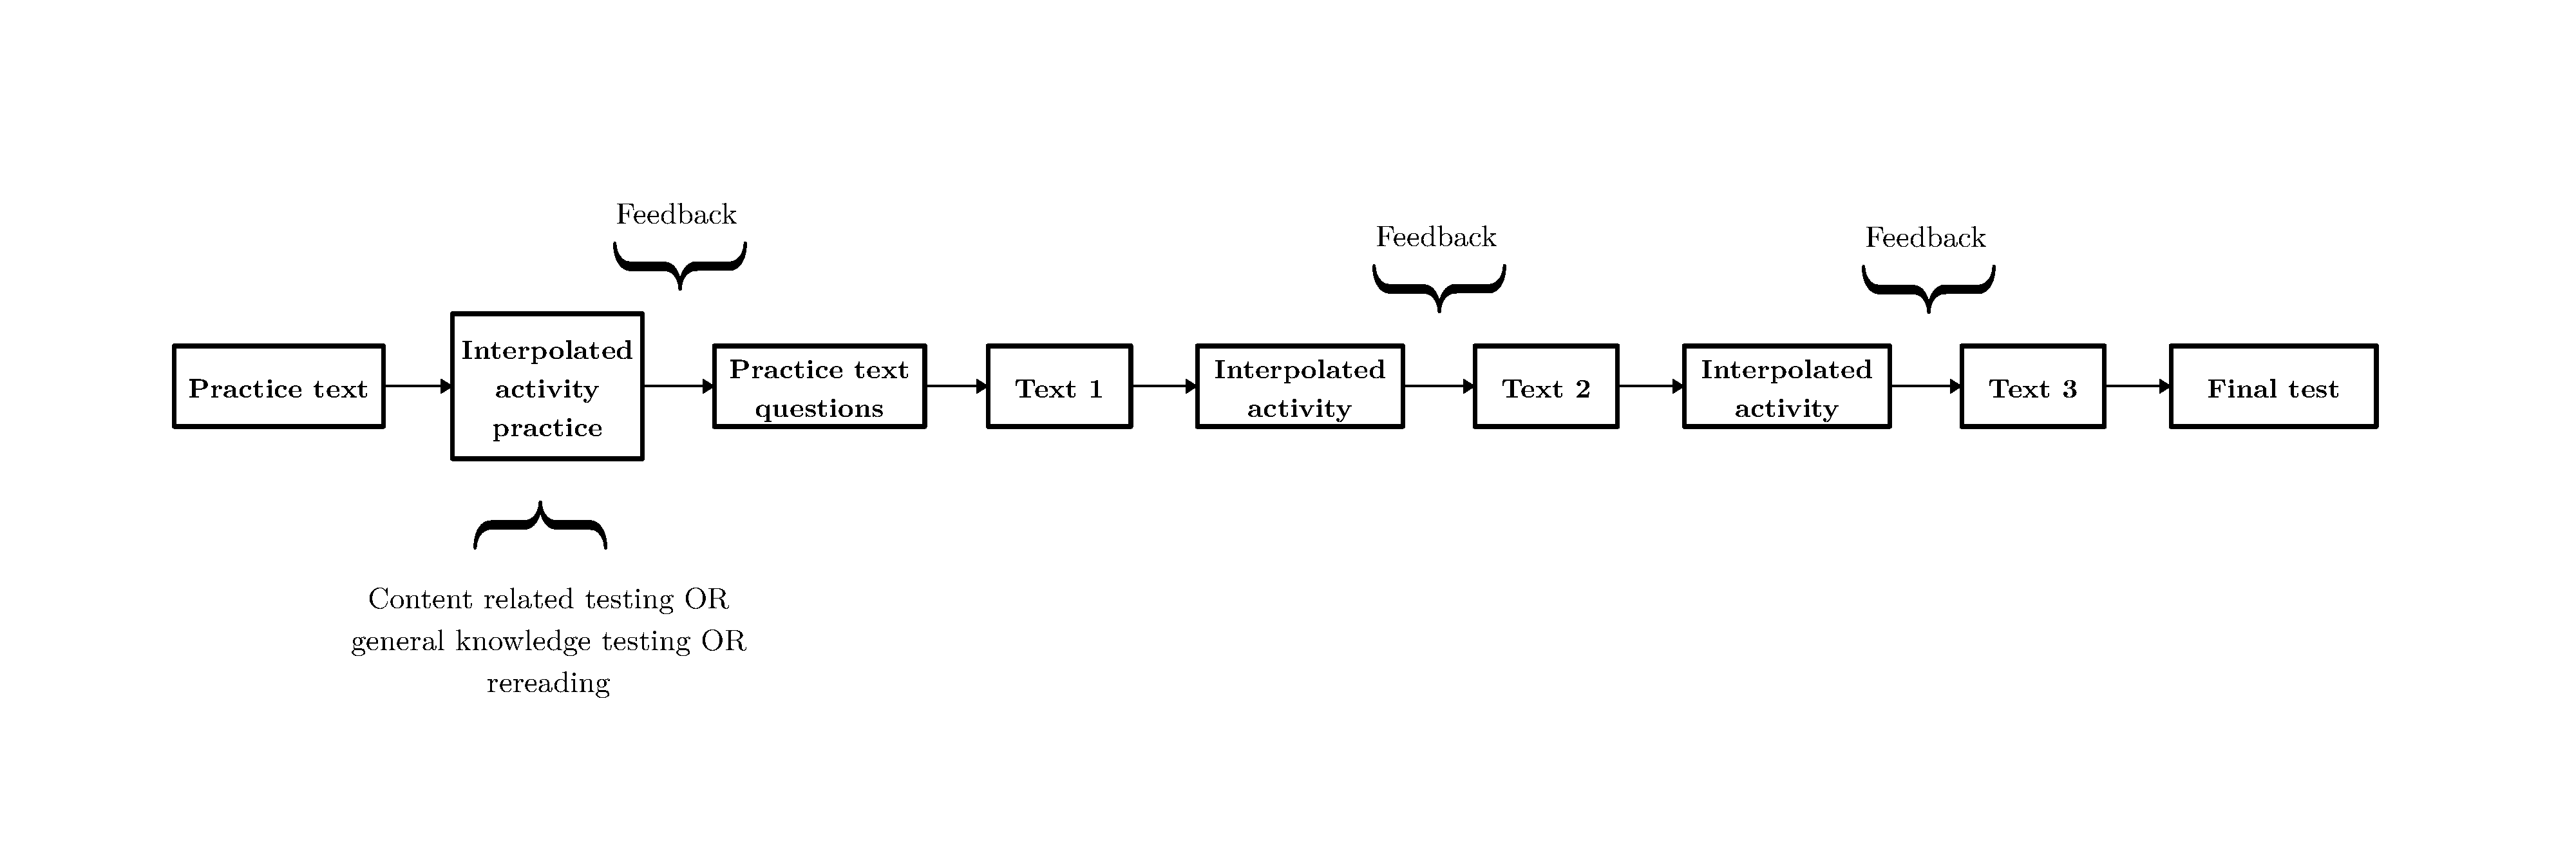
\includegraphics[width = 1.3\textwidth, keepaspectratio, angle = 90, trim = 0 0 0 0]{../images/flowchart/procedure.pdf}
  \caption{A flowchart depicting the experimental procedure.}
  \label{flowchart}
\end{figure}

We will now describe the general procedure. Participants were first
given a brief introduction to the study, and were encouraged to
carefully read and follow the written instructions. Then, they were led
to a computer which was running a fullscreen instance of the
\textit{oTree} application with a randomly chosen experimental
condition. There, participants read the informed consent form and, in
case there were no questions, started the experiment. A flowchart for
the experiment is displayed in Figure \ref{flowchart}.

After entering their personal information, participants were presented
with the instructions for their first task, which was to read the
practice text at a speed that comes naturally to them. Unbeknownst to
the participants, the time they took to read the practice text was
recorded, and used as the basis for determining the reading time limits
for the remaining texts. However, the lowest possible time limit was set
to 5 minutes, and the longest to 8 minutes.

Next, participants were familiarised with the interpolated activity they
were going to perform during the main part of the procedure. The
content-related test group answered four questions based on the practice
text, the general-knowledge test group answered four general knowledge
questions, and the rereading group reread the practice text (this time
with the time limit applied). Subjects in the rereading and general
knowledge conditions also answered the four questions related to the
practice text, in order to familiarise themselves with the scope and
specificity level of the questions they will receive after reading the
final text. Participants assigned to the feedback condition also
received feedback on their interpolated activity practice test
achievement.

After the practice round, participants proceeded to the main part of the
study, engaging in the interpolated activities they were assigned.
Depending on the condition they were assigned to, they also received
feedback after every interpolated test.

All participants were told that there would be a cumulative test after
the final part of the text, examining their knowledge of all three
parts. In reality, the final test examined only the knowledge of the
final part. Participants were presented with twenty questions examining
their knowledge of that part. No feedback was presented after the final
test, irrespective of the experimental condition. The computer recorded
whether a participant correctly answered a question and whether the
participant chose an intrusive distractor. This allowed us to compute
our dependent variables --- the total number of correct answers and the
total number of intrusive distractors chosen.

In total, forty-four content related questions with four response
options were generated from the presented parts of the text. Four
questions were presented after the practice text, ten after each of the
first two parts (only to the participants in the content related test
condition), and twenty after the third part of the text (to all
participants). Starting from the second ten-question-set, the distractor
options were chosen so that (a) two distractors were plausible, but
unrelated to the text, and (b) one distractor was a term or concept
mentioned in the previous part of the text --- this was considered to be
the ``intrusive'' distractor (sometimes reffered to as the ``intrusor''
in the rest of this article). Further, twenty-four general knowledge
questions were generated. These questions were presented to participants
in the general-knowledge test condition, after the first two parts of
the text and after the practice text.


\end{document}
